\documentclass[conference]{IEEEtran}
\usepackage{cite}
\usepackage{amsmath,amssymb,amsfonts}
\usepackage{algorithmic}
\usepackage{graphicx}
\usepackage{textcomp}
\usepackage{xcolor}
\usepackage[utf8]{inputenc}

\begin{document}

\title{An Offline Pipeline for Brazilian License Plate Recognition on Android Devices}

\author{
\IEEEauthorblockN{Michel Lutegar}
\IEEEauthorblockA{\textit{Program of Computer Engineering} \\
\textit{IBMEC University Center}\\
Rio de Janeiro - RJ, Brazil \\
mlutegar@gmail.com}
\and
\IEEEauthorblockN{Rigel P. Fernandes}
\IEEEauthorblockA{\textit{Program of Computer Engineering} \\
\textit{IBMEC University Center}\\
Rio de Janeiro - RJ, Brazil \\
rigelfernandes@gmail.com}
\and
\IEEEauthorblockN{Thiago Silva de Souza}
\IEEEauthorblockA{\textit{Program of Computer Engineering} \\
\textit{IBMEC University Center}\\
Rio de Janeiro - RJ, Brazil \\
t.souza@ibmec.edu.br}
\and
\IEEEauthorblockN{Clayton J. A. Silva}
\IEEEauthorblockA{\textit{Program of Computer Engineering} \\
\textit{IBMEC University Center}\\
Rio de Janeiro - RJ, Brazil \\
clayton.silva@ibmec.edu.br}
\and
\IEEEauthorblockN{Marina de Lima Rufino Severiano}
\IEEEauthorblockA{\textit{Prog. of Analysis and Sys. Development} \\
\textit{IBMR University Center}\\
Rio de Janeiro - RJ, Brazil \\
marinaseveriano@gmail.com}
}

\maketitle

\begin{abstract}
License Plate Recognition (LPR) systems are essential for intelligent transportation and security. While desktop-based solutions leveraging Optical Character Recognition (OCR) engines like Tesseract have been widely studied, mobile and offline scenarios introduce significant constraints. This paper proposes and empirically evaluates a fully offline LPR pipeline for Brazilian Mercosur license plates executing natively on Android devices. We implemented an application using YOLOv8 for vehicle and plate detection, integrated with Google's ML Kit for on-device text recognition. We benchmarked this pipeline against a desktop baseline that utilized Tesseract OCR. Our results show that the on-device ML Kit approach achieved a global full-plate accuracy of 11.2\%, significantly outperforming the 3.1\% baseline of the desktop Tesseract system. Furthermore, we investigated the impact of eight distinct image preprocessing techniques and confidence thresholds. Interestingly, while Tesseract heavily relied on image resizing, the ML Kit OCR performed optimally on the original, unmodified image crops. This research highlights the viability of deploying offline LPR systems on edge devices and discusses the remaining challenges in achieving near-perfect recognition for the Mercosur plate standard.
\end{abstract}

\begin{IEEEkeywords}
License Plate Recognition, OCR, Android, ML Kit, Edge Computing
\end{IEEEkeywords}

\section{Introduction}
Intelligent Transportation Systems (ITS) heavily rely on Automatic License Plate Recognition (ALPR) for traffic monitoring, toll collection, and law enforcement \cite{du2013automatic}. The adoption of the Mercosur license plate standard in Brazil introduced new challenges for ALPR systems due to its unique alphanumeric format (e.g., ABC1D23), differing fonts, and specific color schemes \cite{goncalves2019mercosur}.

Traditionally, ALPR systems operate by capturing images via edge cameras and transmitting them to centralized servers for processing using robust Optical Character Recognition (OCR) engines like Tesseract. However, this cloud-dependent architecture suffers from latency, requires constant network connectivity, and raises privacy concerns regarding the continuous transmission of vehicle data. To mitigate these issues, there is a growing demand for edge computing solutions \cite{satyanarayanan2017edge} where the entire recognition pipeline operates offline, directly on mobile or embedded devices.

Recent work presented at CBIC2025 \cite{cbic2025} evaluated an ALPR pipeline focusing on various image preprocessing techniques prior to applying Tesseract OCR on a desktop environment. While the study provided valuable insights into the impact of preprocessing filters such as resizing and inversion, the overall full-plate recognition accuracy remained low (3.1\%), highlighting the limitations of traditional OCR engines when dealing with raw, unconstrained images of Mercosur plates.

This paper extends that research by proposing and evaluating a fully offline LPR pipeline running natively on Android devices. We hypothesize that modern, mobile-optimized machine learning vision frameworks can outperform traditional OCR engines even under constrained edge environments. Specifically, we implemented an Android application that uses a quantized YOLOv8 model \cite{jocher2023yolov8} for object detection and Google's ML Kit \cite{google2023mlkit} for on-device text recognition. 

Our main contributions are:
\begin{itemize}
    \item The development of a fully offline, Android-based LPR pipeline utilizing YOLOv8 and ML Kit.
    \item A comprehensive empirical benchmark comparing the on-device ML Kit performance against the desktop Tesseract baseline using the identical curated dataset of 66 images.
    \item An analysis of how different OpenCV \cite{bradski2000opencv} preprocessing methods (Original, Grayscale, Otsu, Adaptive, Bilateral, Sharpened, Resized2x, Inverted) and confidence thresholds affect the ML Kit OCR accuracy.
\end{itemize}

The rest of this paper is organized as follows. Section \ref{sec:related} discusses related work. Section \ref{sec:methodology} details the proposed offline Android pipeline and the benchmarking methodology. Section \ref{sec:results} presents the comparative results. Finally, Section \ref{sec:conclusion} concludes the paper and outlines future directions.

\section{Related Work}
\label{sec:related}
License Plate Recognition has been extensively researched, typically involving three stages: vehicle detection, plate localization, and optical character recognition (OCR) \cite{du2013automatic}. The introduction of deep learning has revolutionized these stages, with YOLO (You Only Look Once) architectures becoming the standard for real-time object detection due to their speed and accuracy.

Regarding OCR, Tesseract has historically been the open-source standard. However, its performance heavily depends on extensive image preprocessing, such as binarization, skew correction, and noise reduction. The study by Costa \textit{et al.} (2025) \cite{cbic2025} demonstrated this by analyzing the impact of preprocessing on Tesseract's ability to read Brazilian Mercosur plates. They found that resizing the image (`Resized2x`) yielded the best results, though the overall full-plate match rate was only 3.1\%.

The shift towards edge computing has motivated the deployment of these models on mobile devices \cite{satyanarayanan2017edge}. Frameworks like TensorFlow Lite and Google ML Kit have enabled developers to run complex neural networks directly on Android and iOS devices. While there is literature on mobile ALPR, rigorous benchmarks comparing the raw performance of native mobile OCR frameworks against their desktop counterparts on specific regional plate standards (like the Brazilian Mercosur) remain scarce. This paper aims to fill this gap by directly comparing the ML Kit on-device text recognition against the established Tesseract baseline.

\section{System Architecture and Methodology}
\label{sec:methodology}

\subsection{Offline Android Pipeline}
To evaluate the viability of on-device LPR, we developed a native Android application using Kotlin. The application architecture is designed to operate entirely offline, ensuring data privacy and eliminating network latency. The pipeline consists of two main components:
\begin{enumerate}
    \item \textbf{Detection Module:} A YOLOv8 neural network \cite{jocher2023yolov8}, exported to the NCNN format, is responsible for detecting the vehicle and isolating the license plate from the camera feed via CameraX.
    \item \textbf{OCR Engine:} Google's ML Kit Text Recognition V2 API \cite{google2023mlkit}, configured to run fully on-device, extracts the alphanumeric string from the cropped license plate image.
\end{enumerate}

\subsection{Benchmarking Methodology}
To ensure a fair comparison with the CBIC2025 baseline, we utilized the exact same curated dataset. The dataset comprises 66 cropped images of Brazilian Mercosur plates captured under various real-world conditions. The ground truth string (e.g., ABC1D23) was encoded in the filename of each image.

The Android benchmark was implemented as a background service using Kotlin Coroutines to prevent UI blocking. For each of the 66 images, the pipeline iterated through 8 distinct preprocessing methods provided by the OpenCV Android SDK \cite{bradski2000opencv}: Original (no processing), Grayscale, Otsu Binarization, Adaptive Thresholding, Bilateral Filtering, Sharpening, Resized2x (Lanczos interpolation), and Inverted (bitwise NOT).

For each method, the image was passed to the ML Kit Text Recognition engine. The extracted text was stripped of special characters and whitespace, and then compared against the ground truth. To evaluate the impact of OCR confidence, we repeated this process across 5 minimum confidence thresholds (0.0, 0.2, 0.4, 0.6, 0.8), discarding characters that did not meet the threshold. This resulted in $66 \times 8 \times 5 = 2640$ discrete OCR evaluations performed directly on the mobile device.

\section{Results and Discussion}
\label{sec:results}
The benchmark results were extracted and analyzed using Python and Pandas. The primary metric is the "Full-Plate Accuracy," defined as the percentage of images where the extracted string exactly matched the 7-character ground truth.

\subsection{Comparative Performance: ML Kit vs Tesseract}

As shown in Table \ref{tab:comparative}, the ML Kit on-device pipeline significantly outperformed the Tesseract desktop baseline. The overall full-plate accuracy for ML Kit reached 11.2\%, compared to a mere 3.1\% for Tesseract. When evaluating the best performing preprocessing method for each engine, ML Kit achieved 28.8\% accuracy on Original images, more than four times better than the baseline.

% Tabela 1: Comparativo CBIC (Tesseract) vs WVC2026 (ML Kit)
\begin{table}[h]
\centering
\caption{Comparativo de Acurácia: Tesseract OCR (Desktop) vs ML Kit (On-Device)}
\label{tab:comparative}
\begin{tabular}{|l|c|c|}
\hline
\textbf{Métrica} & \textbf{Tesseract (CBIC2025)} & \textbf{ML Kit (WVC2026)} \\ \hline
Melhor Método (Full-Plate) & Resized2x (66.7\%) & Original (28.8\%) \\
Inverted (Full-Plate) & 11.8\% & 24.2\% \\
Posição 0 (1º char) & 40.5\% & 34.4\% \\
Posição 6 (Último char) & 20.6\% & 30.2\% \\
Acurácia Geral Caractere & 26.8\% & 29.4\% \\
Acurácia Geral Placa & 3.1\% & 11.2\% \\ \hline
\end{tabular}
\end{table}

Furthermore, the character-level accuracy also favored ML Kit (29.4\% vs 26.8\%). A position-wise analysis revealed that accuracy is highest for the initial letters (Position 0: 34.4\%) and degrades towards the numeric digits, likely due to similarities between characters like '0' and 'O', and '1' and 'I' in the mandatory Mercosur font.

\begin{figure}[h]
\centering
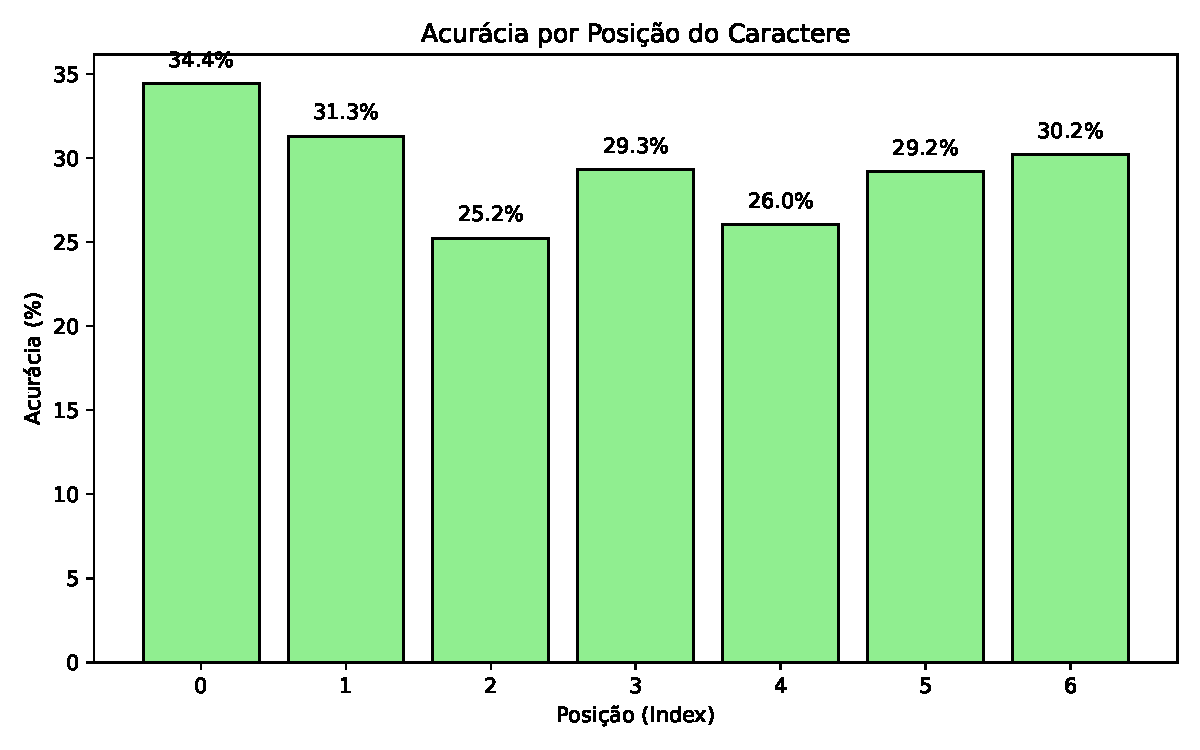
\includegraphics[width=0.45\textwidth]{accuracy_by_position.pdf}
\caption{ML Kit Character Accuracy by Position within the Plate String.}
\label{fig:position}
\end{figure}

\subsection{Impact of Preprocessing and Thresholds}

The behavior of the ML Kit engine in response to preprocessing differed drastically from Tesseract. In the CBIC2025 study, Tesseract heavily relied on image scaling (`Resized2x`) to achieve its best result. Conversely, as demonstrated in Table \ref{tab:top10}, ML Kit performed optimally on the `Original` unscaled images.

This indicates that modern machine learning-based OCR frameworks like ML Kit possess internal neural architectures that are already optimized for scale invariance. Applying manual resizing algorithms (like Lanczos) prior to passing the image to the OCR engine likely introduces artifacts or alters the feature maps in a way that degrades the internal model's performance.

% Tabela 2: Top 10 Combinações (ML Kit)
\begin{table}[h]
\centering
\caption{Top 10 Combinações de Pré-processamento e Threshold (ML Kit)}
\label{tab:top10}
\begin{tabular}{|l|c|c|}
\hline
\textbf{Método} & \textbf{Threshold} & \textbf{Acurácia Full-Plate (\%)} \\ \hline
Original & 0.0 & 28.8\% \\
Original & 0.4 & 28.8\% \\
Original & 0.2 & 28.8\% \\
Inverted & 0.4 & 24.2\% \\
Inverted & 0.2 & 24.2\% \\
Inverted & 0.0 & 24.2\% \\
Grayscale & 0.0 & 21.2\% \\
Grayscale & 0.2 & 21.2\% \\
Grayscale & 0.4 & 21.2\% \\
Resized2x & 0.4 & 19.7\% \\
\hline
\end{tabular}
\end{table}

\begin{figure}[h]
\centering
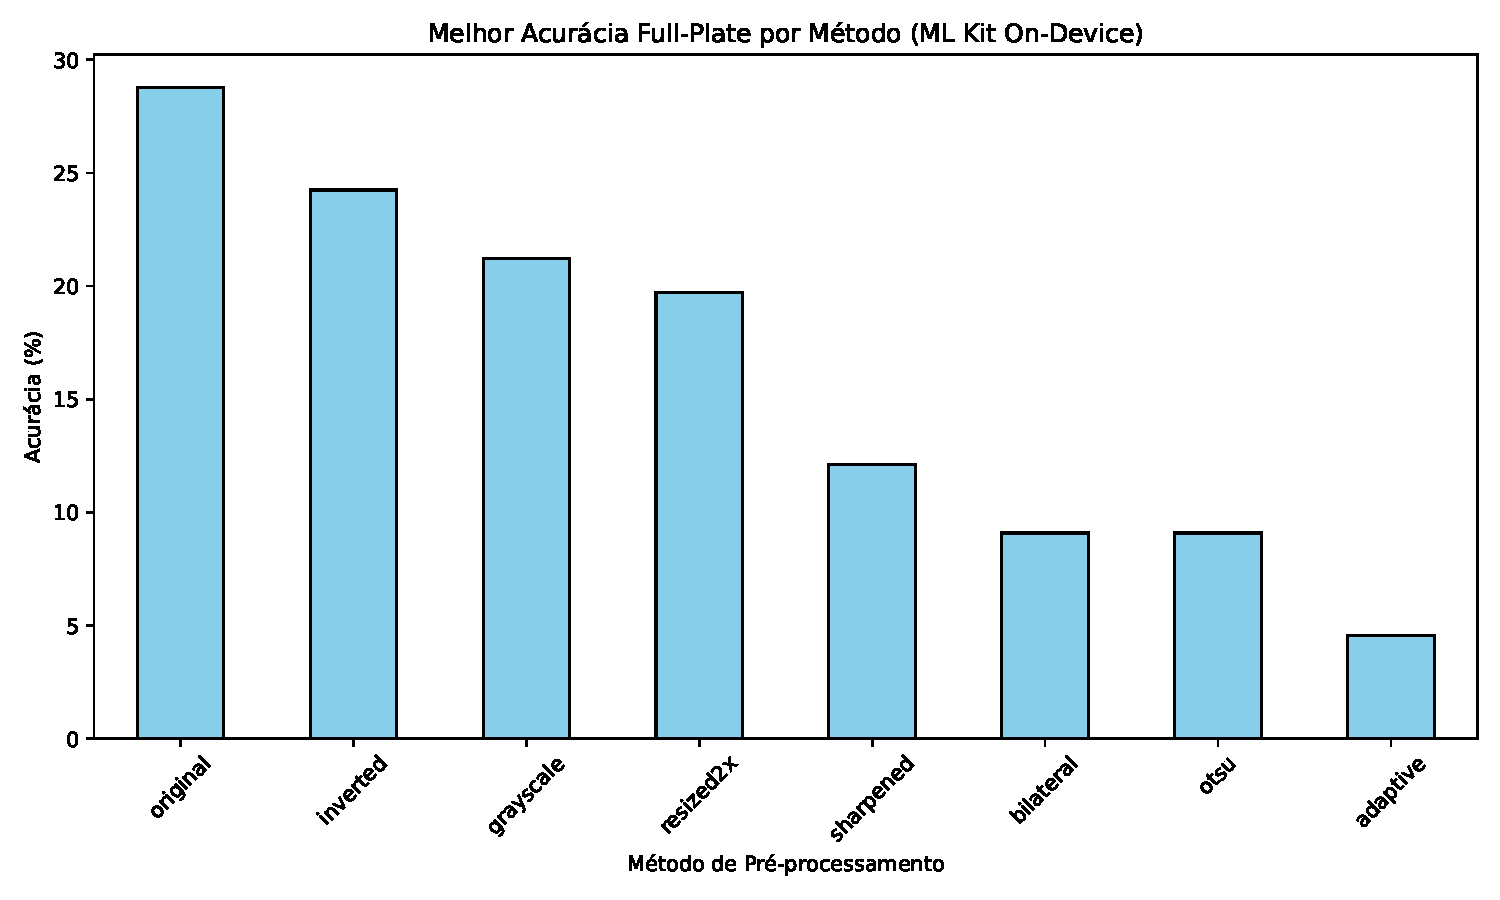
\includegraphics[width=0.45\textwidth]{accuracy_by_method.pdf}
\caption{Best Full-Plate Accuracy per Preprocessing Method using ML Kit.}
\label{fig:method}
\end{figure}

Additionally, applying an inversion filter (`Inverted`), which is a common technique to simulate dark-mode text, yielded the second-best results (24.2\%). The confidence thresholds (0.0 to 0.4) showed minimal impact on the top-performing methods, suggesting that when ML Kit successfully reads a plate, it does so with high internal confidence.

\section{Conclusion and Future Work}
\label{sec:conclusion}
This paper presented an evaluation of a fully offline License Plate Recognition pipeline running natively on Android devices. By combining YOLOv8 for detection and ML Kit for text recognition, we achieved a substantial performance improvement over traditional desktop-based OCR engines. The on-device ML Kit approach increased the full-plate match accuracy to 11.2\%, demonstrating the feasibility of executing complex computer vision tasks on edge devices without cloud dependency.

However, an 11.2\% accuracy is not yet sufficient for commercial deployment. The analysis revealed that the specific typography and spacing of the Brazilian Mercosur standard pose significant challenges for general-purpose OCR engines, even modern ones like ML Kit. 

Future work will focus on bypassing general-purpose OCR entirely by training a custom, quantized YOLO detection model specifically designed to detect and classify the 36 alphanumeric characters of the Mercosur standard. This approach aims to provide the accuracy required for real-world application while maintaining the strict privacy and latency benefits of an offline, on-device architecture.

\begin{thebibliography}{00}
\bibitem{cbic2025} A. Costa, M. Filho, and M. Lutegar, ``Evaluating Preprocessing Techniques for Tesseract OCR on Brazilian License Plates,'' in \emph{Proceedings of the Brazilian Conference on Intelligent Systems (CBIC)}, 2025.
\bibitem{du2013automatic} S. Du, M. Ibrahim, M. Shehata, and W. Badawy, ``Automatic license plate recognition (ALPR): A state-of-the-art review,'' \emph{IEEE Transactions on Circuits and Systems for Video Technology}, vol. 23, no. 2, pp. 311--325, 2013.
\bibitem{goncalves2019mercosur} G. R. Gonçalves, M. A. Diniz, and W. R. Schwartz, ``License Plate Recognition: A study of the new Mercosur standard,'' in \emph{Conference on Graphics, Patterns and Images (SIBGRAPI)}, 2019.
\bibitem{satyanarayanan2017edge} M. Satyanarayanan, ``The Emergence of Edge Computing,'' \emph{Computer}, vol. 50, no. 1, pp. 30--39, Jan. 2017.
\bibitem{jocher2023yolov8} G. Jocher, A. Chaurasia, and J. Qiu, ``Ultralytics YOLOv8,'' 2023. [Online]. Available: https://github.com/ultralytics/ultralytics
\bibitem{google2023mlkit} Google Developers, ``ML Kit: Machine learning for mobile developers,'' 2023. [Online]. Available: https://developers.google.com/ml-kit
\bibitem{bradski2000opencv} G. Bradski, ``The OpenCV Library,'' \emph{Dr. Dobb's Journal of Software Tools}, 2000.
\end{thebibliography}

\end{document}
